%Ultimatives Tool zur Datierung:
%https://www.cc.kyoto-su.ac.jp/~yanom/pancanga/
%skp = ignored in edition
%skm = ignored in xml
\documentclass[10pt]{memoir}
\setstocksize{220mm}{155mm} 	        
\settrimmedsize{220mm}{155mm}{*}	
\settypeblocksize{170mm}{116mm}{*}	
\setlrmargins{18mm}{*}{*}
\setulmargins{*}{*}{1.2}
%\setlength{\headheight}{5pt}%
\checkandfixthelayout[lines]
\linespread{1.16}
\flushbottom

%%% Hyphenation settings
\usepackage[htt]{hyphenat}
\hyphenation{he-lio-trope opos-sum}
\tracingparagraphs=1
%Hyphenation in Devanāgarī of the edition still missing? Probably this needs to be modified in babel-iast package? 

%%% babel
\usepackage[english]{babel}
\usepackage{babel-iast/babel-iast}

\babelfont[iast]{rm}[Renderer=Harfbuzz, Scale=1.3]{AdishilaSan}%AdishilaSan}
\babelfont[english]{rm}{Adobe Text Pro}

%%% more functionality
\PassOptionsToPackage{hyphens}{url}
\usepackage{hyperref}
\usepackage{pdflscape}
\usepackage{cleveref}
\usepackage{url}
\usepackage{cleveref}
\usepackage{microtype}
\usepackage{lineno}

%\usepackage{bigfoot}
%%% more functions
\usepackage[dvipsnames]{xcolor}
%\usepackage[para,perpage]{footmisc}

%%%für den Counter von Kapiteln und Sätzen! 
\newcommand{\uproman}[1]{\uppercase\expandafter{\romannumeral#1}}
\newcommand{\lowroman}[1]{\romannumeral#1\relax}

\makeindex
\newfontfamily\sanskritfont[Script=Devanagari,Mapping=RomDev,Scale=1.1]{Sanskrit2003}
\usepackage{pifont,fourier-orns,lettrine,psvectorian,paralist,enumitem,pdfpages,wrapfig,tabulary,lettrine,longtable}
\setlist[enumerate]{itemsep=0mm}
\usepackage[autostyle]{csquotes}
\usepackage[defaultlines=2,all]{nowidow}
\usepackage{ellipsis,adforn,booktabs,longtable,url,tikz}
\lineskiplimit=-3pt          

\makechapterstyle{IeT}{%
  \chapterstyle{default}
  \renewcommand*{\printchapternonum}{\centering}
  \renewcommand*{\clearforchapter}{\cleartorecto} 
  \aliaspagestyle{chapter}{empty}}
\chapterstyle{IeT}
\setsecnumdepth{none}  \openright  \nouppercaseheads
\settocdepth{subsubsection}

%%%% test better pagebreaks
%\def\fussy{%
%  \emergencystretch\z@
%  \tolerance 200%
%  \hfuzz .1\p@
%  \vfuzz\hfuzz}

%\interfootnotelinepenalty=10000\relax

%\usepackage[maxfloats=256]{morefloats}

%\maxdeadcycles=500

%raggedbottomsectiontrue
%%\checkandfixthelayout


%%%%%%%  biblatex
%\newcommand{\noun}[1]{\textsc{#1}}    %  philosophy-verbose
\usepackage[backend=biber, sorting=nyt, style=verbose]{biblatex} %%%%ORIGINAL TiE
\renewcommand*{\mkbibnamefamily}[1]{\textsc{#1}}


\DeclareFieldFormat{url}{%
  \mkbibacro{URL}\addcolon\space
  \href{#1}{\nolinkurl{\thefield{urlraw}}}}

\DeclareFieldFormat{citeurl}{%
  \href{#1}{\nolinkurl{\thefield{urlraw}}}} 


\DeclareFieldFormat{postnote}{#1}
\renewcommand{\postnotedelim}{, }
\addbibresource{bindu.bib}

%%% ekdosis
\usepackage[teiexport=tidy,parnotes=true]{ekdosis}% =tidy cleans up HTML and XML documents by fixing markup errors and upgrading legacy code to modern standards. parnotes=footnotes below or above critical apparatus

\SetLineation{lineation=page, modulo} %lineation=page sets thenumbering to start afresh at the top of each page. =modulo makes every fifth line numbered. {lineation=page} makes every line numbered! 

\renewcommand{\linenumberfont}{\selectlanguage{english}\footnotesize} %sets language of lines to English

\SetTEIxmlExport{autopar=false} %autopar=falseinstructs ekdosis to ignore blank lines in the.tex sourcefile as markers for paragraph boundaries. As a result, each paragraph of the edition must be found within an environment associated with the xml <p> element

\SetHooks{
  lemmastyle=\bfseries,
  %refnumstyle=\selectlanguage{english}\bfseries,
  refnumstyle=\selectlanguage{english}\color{blue}\bfseries,
  appheight=0.8\textheight,
}

\newif\ifinapparatus
\DeclareApparatus{source}[
%bhook=\inapparatustrue,
lang=english,
notelang=english,
% bhook=\selectlanguage{english},
bhook=\selectlanguage{english}\textbf{Sources:},%
%maxentries=4, 
%ehook=.]
%sep={] },
%nosep,
]

\newif\ifinapparatus
\DeclareApparatus{testium}[
%bhook=\inapparatustrue,
lang=english,
notelang=english,
% bhook=\selectlanguage{english},
bhook=\selectlanguage{english}\textbf{Testimonia:},
%maxentries=4, 
%ehook=.]
%nosep, 
]

% Declare \ifinapparatus and set \inapparatustrue at the beginning of
% the apparatus criticus block. Also set the language.  
\newif\ifinapparatus
  \DeclareApparatus{default}[
  %bhook=\inapparatustrue, 
  lang=english,
  %maxentries=33,
  %bhook=\selectlanguage{english},
  sep = {] },
  delim=\hskip 0.75em,
  rule=\rule{0.7in}{0.4pt},
]

\newif\ifinapparatus
\DeclareApparatus{philcomm}[
%bhook=\inapparatustrue,
lang=english,
notelang=english,
bhook=\selectlanguage{english}\textbf{Philological Commentary:},
%bhook=\selectlanguage{english},
sep={: },
]

\ekdsetup{
showpagebreaks,
spbmk = \textcolor{blue}{spb},
hpbmk = \textcolor{red}{hpb}
}

%\usepackage{fnpos}
%\makeFNmid
%\makeFNbottom
\usepackage[bottom]{footmisc}
%%%%%%%%%%%%%%%%%%%%%%%%%%%
\makeatletter
\def\blfootnote{\gdef\@thefnmark{}\@footnotetext}
\makeatother
%%%%%%%%%%%%%%%%%%%%%%%%%


% Macros and Definitions for the Print of Sigla
\def\acpc#1#2#3{{#1}\rlap{\textrm{\textsuperscript{#3}}}\textsubscript{\textrm{#2}}\space}
\def\sigl#1#2{{{#1}}\textsubscript{\textrm{#2}}}
\def\None{{\sigl{N}{1}}} \def\Noneac{\acpc{N}{1}{ac}\,} \def\Nonepc{\acpc{N}{1}{pc}\,}
\def\Ntwo{{\sigl{N}{2}}} \def\Noneac{\acpc{N}{2}{ac}\,} \def\Nonepc{\acpc{N}{2}{pc}\,}
\def\Done{{\sigl{D}{1}}} \def\Doneac{\acpc{D}{1}{ac}\,} \def\Donepc{\acpc{D}{1}{pc}\,}
\def\Dtwo{{\sigl{D}{2}}} \def\Dtwoac{\acpc{D}{2}{ac}\,} \def\Dtwopc{\acpc{D}{2}{pc}\,}
\def\Uone{{\sigl{U}{1}}} \def\Uoneac{\acpc{U}{1}{ac}\,} \def\Uonepc{\acpc{U}{1}{pc}\,}                 
\def\Utwo{{\sigl{U}{2}}} \def\Utwoac{\acpc{U}{2}{ac}\,} \def\Utwopc{\acpc{U}{2}{pc}\,}

%%%%%%%%%%%%%% Tattvabinduyoga - List of Witnesses   %%%%%%%%%%%%%%%%%%%
\DeclareWitness{ceteri}{\selectlanguage{english}cett.}{ceteri}[]   
\DeclareWitness{E}{\selectlanguage{english}E}{Printed Edition}[]    
\DeclareWitness{P}{\selectlanguage{english}P}{Pune BORI 664}[]  
\DeclareWitness{B}{\selectlanguage{english}B}{Bodleian 485}[]       
\DeclareWitness{N1}{\selectlanguage{english}N\textsubscript{1}}{NGMPP 38/31}[]
\DeclareWitness{N2}{\selectlanguage{english}N\textsubscript{2}}{NGMPP B 38/35}[]
\DeclareWitness{L}{\selectlanguage{english}L}{LALCHAND 5876}[]  
\DeclareWitness{D}{\selectlanguage{english}D}{IGNCA 30019}[] 
%\DeclareWitness{D2}{\selectlanguage{english}D\textsubscript{2}}{IGNCA 30020}[]  
\DeclareWitness{U1}{\selectlanguage{english}U\textsubscript{1}}{SORI 1574}[] 
\DeclareWitness{U2}{\selectlanguage{english}U\textsubscript{2}}{SORI 6082}[]
%%%%%%%%%%%%%% Tattvabinduyoga - Groups of Witnesses   %%%%%%%%%%%%%%%%%%%
\DeclareWitness{X}{\selectlanguage{english}\alpha}{Alpha Group: D,N1,N2,U1}[]
\DeclareWitness{Y}{\selectlanguage{english}\beta}{Beta Group: B,E,L,P,U2}[]
%%%%%%%%%%%%% Testimonia
\DeclareWitness{Ysv}{\selectlanguage{english}Ysv}{Yogasvarodaya}[] %%%add infos!  

%%%%%%%%%%%%%%%%%%%%%%%%%%%%%%%%%%%%%%%%%%%
% Macro for Editing Abbrevs.
\def\om{\textrm{\footnotesize \textit{om.}\ }} %prints om. for omitted in apparatus
\def\korr{\textrm{\footnotesize \textit{em.}\ }} %prints em. for emended in apparatus
\def\conj{\textrm{\footnotesize \textit{conj.}\ }} %prints conj. for conjectured in apparatus

% \supplied{text} EDITORIAL ADDITION -> Within \lem oder \rdg
% \surplus{text} EDITORIAL DELETION -> Within \lem oder \rdg
% \sic{text} CRUX
% \gap{text} LACUNAE -> [reason=??, unit=??, quantity=??, extent=??]


%%%%%%%%%%%%%%%%%%%%%%%%%%%%%%%%%%%%%%%%%%% All macros of this list can be used in 
% Macro for Editing Abbrevs.
\def\eyeskip{\textrm{{ab.\,oc. }}}
\def\aberratio{\textrm{{ab.\,oc. }}}
\def\ad{\textrm{{ad}}}
\def\add{\textrm{{add.\ }}}
\def\ann{\textrm{{ann.\ }}}
\def\ante{\textrm{{ante }}} 
\def\post{\textrm{{post }}}
%\def\ceteri{cett.\,}                   
\def\codd{\textrm{{codd.\ }}}

\def\coni{\textrm{{coni.\ }}}
\def\contin{\textrm{{contin.\ }}}
\def\corr{\textrm{{corr.\ }}}
\def\del{\textrm{{del.\ }}}
\def\dub{\textrm{{ dub.\ }}}

\def\expl{\textrm{{explic.\ }}} 
\def\explica t{\textrm{{explic.\ }}}
\def\fol{\textrm{{fol.\ }}}
\def\foll{\textrm{{foll.\ }}}
\def\gloss{\textrm{{glossa ad }}}
\def\ins{\textrm{{ins.\ }}}      
\def\inseruit{\textrm{{ins.\ }}} 
\def\im{{\kern-.7pt\lower-1ex\hbox{\textrm{\tiny{\emph{i.m.}}}\kern0pt}}} %\textrm{\scriptsize{i.m.\ }}}      
\def\inmargine{{\kern-.7pt\lower-.7ex\hbox{\textrm{\tiny{\emph{i.m.}}}\kern0pt}}}%\textrm{\scriptsize{i.m.\ }}}      
\def\intextu{{\kern-.7pt\lower-.95ex\hbox{\textrm{\tiny{\emph{i.t.}}}\kern0pt}}}%\textrm{\scriptsize{i.t.\ }}}           
\def\indist{\textrm{{indis.\ }}}  
\def\indis{\textrm{{indis.\ }}}
\def\iteravit{\textrm{{iter.\ }}} 
\def\iter{\textrm{{iter.\ }}}
\def\lectio{\textrm{{lect.\ }}}   
\def\lec{\textrm{{lect.\ }}}
\def\leginequit{\textrm{{l.n. }}} 
\def\legn{\textrm{{l.n. }}}
\def\illeg{\textrm{{l.n. }}}

\def\primman{\textrm{{pr.m.}}}
\def\prob{\textrm{{prob.}}}
\def\rep{\textrm{{repetitio }}}
\def\secundamanu{\textrm{\scriptsize{s.m.}}}            \def\secm{{\kern-.6pt\lower-.91ex\hbox{\textrm{\tiny{\emph{s.m.}}}\kern0pt}}}%   \textrm{\scriptsize{s.m.}}}
\def\sequentia{\textrm{{seq.\,inv.\ }}}  
\def\seqinv{\textrm{{seq.\,inv.\ }}}
\def\order{\textrm{{seq.\,inv.\ }}}
\def\supralineam{{\kern-.7pt\lower-.91ex\hbox{\textrm{\tiny{\emph{s.l.}}}\kern0pt}}} %\textrm{\scriptsize{s.l.}}}
\def\interlineam{{\kern-.7pt\lower-.91ex\hbox{\textrm{\tiny{\emph{s.l.}}}\kern0pt}}}   %\textrm{\scriptsize{s.l.}}}
\def\vl{\textrm{v.l.}}   \def\varlec{\textrm{v.l.}} \def\varialectio{\textrm{v.l.}}
\def\vide{\textrm{{cf.\ }}}
\def\cf{\textrm{{cf.\ }}} 
\def\videtur{\textrm{{vid.\,ut}}}
\def\crux{\textup{[\ldots]} }
\def\cruxx{\textup{[\ldots]}}
\def\unm{\textit{unm.}}
%%%%%%%%%%%%%%%%%%%%%%%%%%%%%%%%%%%%

% List of Scholars
\DeclareScholar{ego}{ego}[
forename=Nils Jacob,
surname=Liersch]

% Persons:14\DeclareScholar{ego}{ego}[15forename=Robert,16surname=Alessi]17% Useful shorthands:18\DeclareShorthand{codd}{codd.}{V,I,R,H}19\DeclareShorthand{edd}{edd.}{Lit,Erm,Sm}20\DeclareShorthand{egoscr}{\emph{scripsi}}{ego}

%Useful shorthands:
%\DeclareShorthand{codd}{codd.}{V,I,R,H}
%\DeclareShorthand{edd}{edd.}{Lit,Erm,Sm}
\DeclareShorthand{egoscr}{em.}{ego}
\DeclareShorthand{egoscrconj}{conj.}{ego}
\DeclareShorthand{egomute}{\unskip}{ego}

\usepackage{xparse}

\NewDocumentEnvironment{tlg}{O{}O{}}{\setlength{\leftskip}{0pt}\vspace{-1ex}\begin{quotation}}{\hfill #1\ \vspace{-1ex}\end{quotation}\vspace{-1ex}} %verse environment
%\NewDocumentEnvironment{tlg}{O{}O{}}{\begin{verse}}{॥#1\hskip-4pt ॥\\ \end{verse}}
\NewDocumentCommand{\tl}{m}{{\selectlanguage{iast} #1}}

\NewDocumentCommand{\extra}{m}{{\textcolor{gray}{#1}}} %command for additions to U2
\NewDocumentCommand{\crazy}{m}{{\textcolor{red}{#1}}} %totally corrupted passage
\NewDocumentCommand{\coro}{m}{{\textcolor{violet}{#1}}} %colour for sentence counter! 

\NewDocumentEnvironment{prose}{O{}}{\begin{otherlanguage}{iast}}{\end{otherlanguage}}
% \NewDocumentEnvironment{padd}{O{}}{\begin{otherlanguage}{iast}}{\end{otherlanguage}}
\NewDocumentEnvironment{tlate}{O{}}
%\NewDocumentEnvironment{tadd}{O{}}

%Define two commands: \skp ("sanskrit plus"), to be ignored by TeX in
%the edition text, but processed in the TEI output. Conversely, \skm
%("sanskrit minus") is to be processed in the edition text, but
%ignored if found in the apparatus criticus and in the TEI output:

\NewDocumentCommand{\skp}{m}{}
\TeXtoTEIPat{\skp {#1}}{#1}

%\NewDocumentCommand{\skpp}{m}{}
%\TeXtoTEIPat{\skpp {#1}}{#1}

\NewDocumentCommand{\skm}{m}{\unless\ifinapparatus#1-\fi}
\TeXtoTEIPat{\skm {#1}}{}

% \NewDocumentCommand{\dd}{}{/\hskip-4pt/}
\NewDocumentCommand{\dd}{}{\mbox{/\hskip-4pt/}}
\TeXtoTEIPat{\dd {}}{//}


%%% modify environments and commands
%%% TEI mapping
\TeXtoTEIPat{\begin {tlg}}{<lg>} %lg=(Group of verse (s)) contains one or more verses or lines of verse that together form a formal unit (e.g. stanza, chorus).
\TeXtoTEIPat{\end {tlg}}{</lg>}

\TeXtoTEIPat{\begin {prose}}{<p>}
\TeXtoTEIPat{\end {prose}}{</p>}

\TeXtoTEIPat{\begin {tlate}}{<p>}
\TeXtoTEIPat{\end {tlate}}{</p>}

\TeXtoTEIPat{\\}{}
\TeXtoTEIPat{\linebreak}{<br/>}
\TeXtoTEIPat{\noindent}{}
%\TeXtoTEI{tl}{l}
\TeXtoTEI{emph}{hi}
\TeXtoTEI{bigskip}{}
\TeXtoTEI{None}{N1}
\TeXtoTEI{Ntwo}{N2}
\TeXtoTEI{Done}{D1}
\TeXtoTEI{Dtwo}{D2}
\TeXtoTEI{Uone}{U1}
\TeXtoTEI{Utwo}{U2}
%\TeXtoTEIPat{/}{ |}
%\TeXtoTEI{//}{ ||}
\TeXtoTEIPat{\korr}{em. }
\TeXtoTEIPat{\conj}{conj.}
\TeXtoTEIPat{\om}{om.}
\TeXtoTEIPat{english}{}
\TeXtoTEIPat{\hskip}{}
\TeXtoTEIPat{\hskip-4pt}{}
\TeXtoTEIPat{\hskip-2pt}{}
\TeXtoTEIPat{-}{ }
\TeXtoTEIPat{4pt}{}
\TeXtoTEIPat{2pt}{}
\TeXtoTEIPat{\textcolor {#1}{#2}}{<hi rend="#1">#2</hi>} 

% Nullify \selectlanguage in TEI as it has been used in
% \DeclareWitness but should be ignored in TEI.
\TeXtoTEI{selectlanguage}{}



\FormatDiv{1}{\begin{center}\Large}{\end{center}}
\FormatDiv{2}{\begin{center}\small}{\end{center}}
\FormatDiv{3}{\bfseries}{.}
\title{Tattvayogabindu of Rāmacandra\\ A Critical Edition and Annotated Translation\\ and a Comparative Analysis of the \\Complex Early Modern Yoga Yaxonomies }
\date{\today}
\parindent=15pt

\begin{document}

\frontmatter
\thispagestyle{empty} % Verhindert Seitenzahl auf der Seite
\begin{center}

%\vspace{0.5in}

%\begin{otherlanguage}{iast}
%   \large\sanskritfont{Tattvayogabindu}\\
%\end{otherlanguage}

\vspace{0.25in}


\huge\textbf{\MakeUppercase{The Tattvayogabindu \\of Rāmacandra}}\\

\vspace{0.2in}

\Large  Critical Edition and Annotated Translation of an Early Modern Text on Rājayoga, with a Comparative Analysis of the Complex Yoga Taxonomies from the Same Period\\ 

\vspace{0.45in}

\thispagestyle{empty}
\end{center}
%\newpage
%\thispagestyle{empty}
%\mbox{}
%\newpage

\newpage

  \thispagestyle{empty}
  \begin{figure}[p]
    \centering
    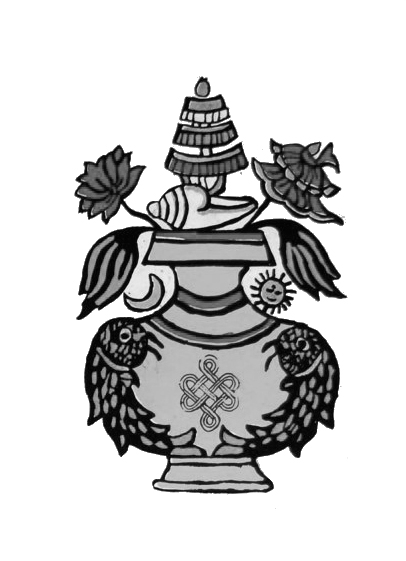
\includegraphics[width=0.25\textwidth]{pics/purna.jpg}
  \end{figure}
  
\newpage

\begin{landscape}
\thispagestyle{empty}
  \begin{figure}[p]
	\centering
  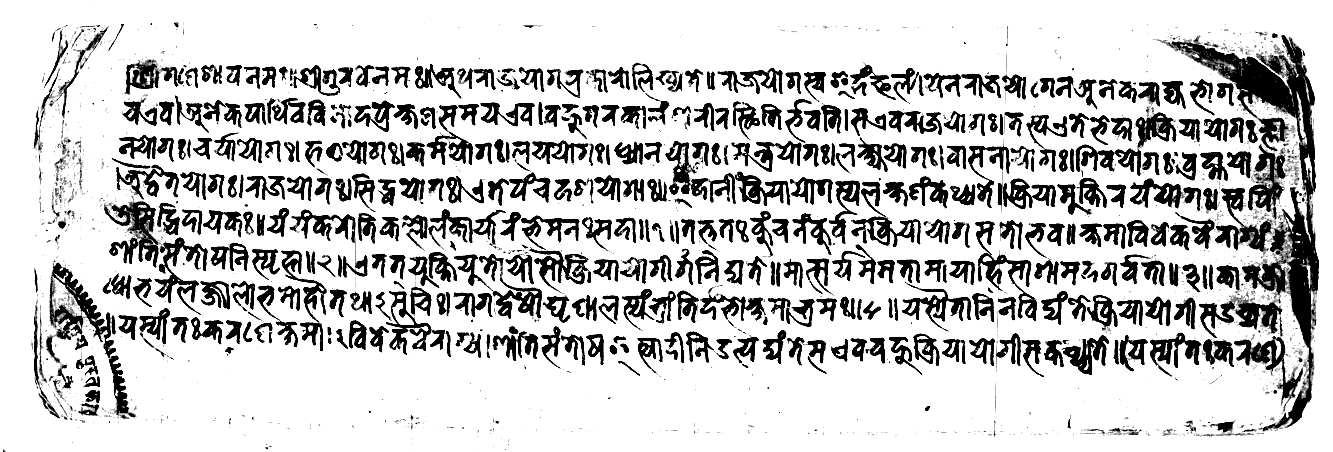
\includegraphics[width=1.5\textwidth]{pics/folio1.jpg}
	\caption{Folio 1v of Ms. \getsiglum{N1}.}
	 \phantomsection\label{fig_folio1}
\end{figure}
\end{landscape}

\cleardoublepage
\tableofcontents
\thispagestyle{empty}
\newpage 
\listoffigures
\thispagestyle{empty}
\newpage
\listoftables
\thispagestyle{empty}
\newpage

\mainmatter
\pagestyle{defaultstyle}
\counterwithout{footnote}{chapter}
\counterwithout{figure}{chapter}
\counterwithout{table}{chapter}
\renewcommand{\thetable}{\arabic{table}}
%%%tables 
\setsecnumdepth{section}
\maxsecnumdepth{subsubsection}
\newpage
\chapter{Introduction}
\cleardoublepage

\section{General remarks}
 \phantomsection\label{generalremarks}
 \lettrine{T}{he} \textit{Tattvayogabindu} of Rāmacandra\footnote{A discussion about the author Rāmacandra is found on p. \pageref{ramarama}.} is an early modern Sanskrit text on Rājayoga that was written in the first half of the seventeenth century\footnote{The dating of the text is discussed on p. \pageref{dating}.} in northern India.\footnote{The detailed discussion of the place of origin is found on p. \pageref{riversrivers}, n. \ref{riversrivers}.} The most salient feature of the work that makes it historically significant is its highly differentiated taxonomy of types of yoga.\footnote{This is a remarkable increase in the number of declared yogas compared to the standard medieval tetrad of Mantra, Laya, Haṭha and Rājayoga.} In the \textit{Tattvayogabindu}'s introduction, most manuscripts name fifteen types of yoga, presented as methods of Rājayoga. These are 1. Kriyāyoga, 2. Jñānayoga, 3. Caryāyoga, 4. Haṭhayoga, 5. Karmayoga, 6. Layayoga, 7. Dhyānayoga, 8. Mantrayoga, 9. Lakṣyayoga, 10. Vāsanāyoga, 11. Śivayoga, 12. Brahmayoga, 13. Advaitayoga, 14. Siddhayoga, and 15. Rājayoga itself. The text is a yogic compendium written in a mix of mainly prose and 47 verses in textbook-style, where its 59 topics are introduced in sections most of the time launched by recognizable phrases. The sections deal with the methods of Rājayoga and their effects, but others also cover topics like yogic physiology, the Avadhūta, the importance of the guru, cosmogony, and a \textit{yogaśāstrarahasya}.  

The \textit{Tattvayogabindu} has not been discussed comprehensively or considered in the secondary literature on yoga. The only exception is \citeauthor{birch2014} (2014: 415–416) who briefly described its list of fifteen yogas in the context of the ``fifteen medieval yogas'' and noted that a similar taxonomy occurs in Nārāyaṇatīrtha’s \textit{Yogasiddhāntacandrikā} (17th century), a commentary on the \textit{Pātañjalayogaśāstra} that integrates fifteen medieval yogas within its \textit{aṣṭāṅga} format. An incomplete account of the fifteen yogas is found within the Sanskrit yoga text \textit{Yogasvarodaya}, which is known only through quotations in the \textit{Prāṇatoṣinī}, the \textit{Yogakarṇikā} and the \emph{Śabdakalpadruma}.\footnote{Manuscripts under the name of \textit{Yogasvarodaya} seem to be lost. I was not able to locate the manuscripts of the text in any manuscript catalogue at hand.} The \textit{Yogasvarodaya} announces a total of fifteen yogas but names only eight of them in its introductory \textit{śloka}s. It is the primary source and template for the compilation of the \textit{Tattvayogabindu}. Besides several passages, Rāmacandra, in many instances, follows its content and structure by rewriting the \textit{Yogasvarodaya}’s \textit{śloka}s into prose or quoting them directly without attribution. Due to the incomplete transmission of the \textit{Yogasvarodaya}, Rāmacandra’s \textit{Tattvayogabindu} is a natural and valuable starting point for an unprecedented in-depth study of the complex early modern yoga taxonomies, a phenomenon that can be narrowed down precisely in terms of time and as I will show regarding its localisation. The other source text that Rāmacandra used is the \textit{Siddhasiddhāntapaddhati} whose content he draws on, particularly in the second half of his composition. Another text that includes an almost similar taxonomy of twelve yogas divided into three tetrads\footnote{See p.\pageref{sarvasarva} for a detailed discussion of the \textit{Sarvāṅgayogapradīpikā}.} is Sundardās’s \textit{Brajbhāṣā} yoga text named \textit{Sarvāṅgayogapradīpikā} which not just shares most of the types of yogas but also provides a different and valuable perspective on the addressed yoga categories.\footnote{For a comparative table of the complex early modern yoga taxonomies see table \ref{tab:complextaxonomies} on p. \pageref{tab:complextaxonomies}.}

These complex taxonomies that emerged during the 17th century crossed sectarian divides and were adapted to the specific needs of different authors and traditions. The \textit{Tattvayogabindu} thus encapsulates a large proportion of the diversity of yoga types and teachings after the \textit{Haṭhapradīpikā} (15th century) that were adopted and practised by a broad spectrum of religious traditions and strata of Indian society. In the particular case of the \textit{Tattvayogabindu}, there are various statements throughout the text that reveal a strategy to detach yoga from its ascetic and renunciate connotations and to stylise Rājayoga as a practice that can bring the desired soteriological benefits even to practitioners who enjoy worldly pleasures and expensive lifestyles. Textual evidence suggests that the \textit{Tattvayogabindu} is an important example of a text that provides an early modern adaptation of Rājayoga for \textit{kṣatriya}s in a courtly environment.

One printed edition of the \textit{Tattvayogabindu} was published in 1905 with a Hindi translation and based on (an) unknown manuscript(s).\footnote{\emph{Binduyoga}. \textit{Binduyogaḥ with Bhāṣaṭīkā}. Ed. by Jvālāprasāda Miśra. Mumbai, 1905.} This publication has the title ``\textit{Binduyoga}'' confirmed by the printed text’s colophon. However, as I will discuss in the introduction, the text was originally known as \textit{Tattvayogabindu}. The consulted manuscripts contain significant discrepancies, structural differences and variant readings between them and the printed edition.\footnote{For example, the printed edition does not contain the complex yoga taxonomy presented in the manuscripts of the \emph{Tattvayogabindu}.} Furthermore, the manuscripts are scattered over the northern half of the Indian subcontinent and Nepal, which suggests that the text was widely transmitted at some point. Lengthy passages of the \textit{Tattvayogabindu} are quoted without attribution in a text called \textit{Yogasaṃgraha} and Sundaradeva’s \textit{Haṭhasaṅketacandrikā}.

The first chapter of this dissertation contains a general introduction to Rāmacandra's \textit{Tattvayogabindu}. The chapter gives a brief overview of the content of the text and discusses its origin, the author and the author's intended audience. Subsequently, the textual witnesses, source texts and testimonies of the \textit{Tattvayogabindu} are described. A stemmatic analysis of the text is then presented, based on manual philological observation and computer-assisted stemmatics to present a \textit{stemma codicum}. The chapter concludes with a presentation of the editorial policies, which form the basis for the second chapter of this thesis.
The second chapter, the core of this dissertation, is a critical edition and annotated translation of the \textit{Tattvayogabindu}. The critical edition significantly improves the text and sheds new light on its historical significance.
The third chapter contains a comparative analysis of the complex early modern yoga taxonomies based on hermeneutics of difference.\footnote{The conceptof hermeneutics of difference is discussed on p. \pageref{hermeneutics}, n. \ref{hemerneutics}.}  Using the new critical edition of the \textit{Tattvayogabindu} and the texts mentioned above, \emph{Yogasvarodaya}, \emph{Yogasiddhāntacandrikā} and \emph{Sarvāṅgayogapradīpikā}, the complex yogic taxonomies of the four texts are compared in detail. Based on this comparative analysis, a differentiated hypothesis on the emergence of the complex yoga taxonomies was developed, and the complex yoga taxonomies were located und explained in the broader context of the historical development of the yoga traditions. The comparison includes a nuanced description of each yoga category used by the authors of the texts with complex yoga taxonomies. While the authors of the four texts often operate with identical terms for the individual yoga categories, they interpret these categories according to their religious backgrounds and agendas, with intriguing and exciting differences. Contrasting the comparanda, i.e. the authors, the texts, the yoga taxonomies and the yoga categories, therefore provides a deep insight into the discursive negotiation processes of the Indian yoga traditions of the 17th century.


\chapter{Conventions in the Critical Apparatus}
\section{Sigla in the Critical Apparatus}

\begin{itemize}
\item \beta : \getsiglum{D}, \getsiglum{J}, \getsiglum{K1}, \getsiglum{N1}, \getsiglum{N2}, \getsiglum{U1}
\item \gamma : \getsiglum{B}, \getsiglum{E}, \getsiglum{L}, \getsiglum{P}, \getsiglum{U2}
\item B : Bodleian Oxford D 4587
\item C : \emph{Haṭhasaṅketacandrikā} GOML Ms. No. R 3239
\item C\textsubscript{pc} : \emph{Haṭhasaṅketacandrikā} GOML Ms. No. R 3239
\item cett.: ceteri (all manuscripts except the ones mentioned in the lemma)
\item \Done : IGNCA 30019
\item E : Printed Edition
\item J : JNUL Ms. No. 55769
\item Jo : \emph{Haṭhasaṅketacandrikā} MMPP MS. No. 2244
\item \Kone : AS G 11019
\item L : Lalchand Research Library LRL5876
\item M : \emph{Haṭhasaṅketacandrikā} ORI Ms. No. B 220
\item \Ntwo : NGMPP B 38-35 / A 1327-14
\item \None : NGMPP B 38-31
\item P : Pune BORI 664
\item PT : \emph{Prāṇatoṣiṇī}
\item \Uone : SORI 1574
\item \Utwo : SORI 6082
\item V : OI MSU 10558
\item YK : \emph{Yogakarṇikā}% 
\item YSv : \emph{Yogasvarodaya}
\end{itemize}
\newpage

\chapter[Critical Edition \& Annotated Translation of the \emph{Tattvayogabindu}]{The \emph{Tattvayogabindu} of Rāmacandra \\ \huge  
  Critical Edition \& Annotated Translation}
\pagestyle{chapter2style}
\clearpage
\begin{alignment}[
  texts=edition[class="edition"];
  translation[class="translation"],
  ]
  \begin{edition}
                   \ekddiv{
                     head={[\uproman{16}. \textbf{rājayogayuktasya puruṣasya yac charīracihnam}]},
                     type=section,
                     depth=2, 
                     n=XVI
                   }
                   \xmlhead[h16]{[XVI. rājayogayuktasya puruṣasya yac charīracihnam]}
                   \phantomsection
                   \addcontentsline{toc}{section}{XVI. rājayogayuktasya puruṣasya yac charīracihnam}
                  \phantomsection\label{rajabody}
                      \begin{prose}[p16_01]
      \noindent
%------------------------------  
%idānīṃ rājayogayuktasya           śarīre yaccihnaṃ  tat    kathyate / \E
%idānīṃ rājayogayuktasya puruṣasya yaccharīracihnaṃ         kathyate / \P
%idānīṃ rājayogayuktasya puruṣasya          cinhnaṃ         kathyate / \L
%idānīṃ rājayogayuktasya puruṣasya          cinhnaṃ         kathyate // \B
%idānīṃ rājayogayuktasya puruṣasya yaccarīracihnaṃ   tat    kathyate / \N1
%idānīṃ rājayogayuktasya puruṣasya yaccharīracihūṃ   tat    kathyate// \N2
%idānīṃ rājayogayuktasya puruṣasya yaccarīracihnaṃ   tat    kathyate / \D
%idānīṃ rājayogayuktasya puruṣasya yacharīre cihnaṃ   tat    kathyate // \J
%idānīṃ rājayogayuktasya puruṣasya yaccarīracihnaṃ   tat    kathyataṃ / \K1      
%idānīṃ rājayogayuktasya puruṣasya yaccharīre cinhaṃ tata   kathyate \U1
%idānīṃ rājayogayuktasya puruṣasya yat śarīracinhaṃ         kathyate / \U2
%------------------------------
%Now, the sign of the body of the person who is endowed with Rājayoga is taught.
%------------------------------    
\note[type=source, labelb=_39b, labele={_39e}, nosep]{cf. YSv (PT, p. 834): idānīṃ kathayiṣyāmi rājayogasya lakṣaṇam | rājayoge kṛte puṃbhiḥ siddhicihnaṃ bhaved iti | paripūrṇaṃ bhavec cittaṃ jagatstho 'pi jagadbahiḥ | na kṣobho janma mṛtyuś ca na duḥkhaṃ na sukhaṃ tathā | bhedābhedau manaḥsthau na jñānaṃ śīlaṃ kulaṃ tathā | prakāśakuśasambandhiprasaṅgo 'yaṃ nirantaram | sarvaprakāśako 'sau tu naṣṭabhedādir eva ca | asya citte nānurāgo virāgo na bhaved iti | asya jāter na cihnañ ca niṣkalo 'yaṃ nirañjanaḥ | ananto 'yaṃ mahājyotir vāñchāṃ bhogaṃ dadāti ca |}
idānīṃ rājayogayuktasya
  \app{\lem[wit={ceteri}]{puruṣasya}\linelabel{_39b}
    \rdg[wit={E}]{\om}}
  \app{\lem[wit={D,N1,P},alt={yac charīracihnaṃ}]{yaccharīracihnaṃ}
    \rdg[wit={K1}]{yaccharīracihnaṃ}
    \rdg[wit={E}]{śarīre yac cihnaṃ}
    \rdg[wit={U1}]{yac charīre cinhaṃ}
    \rdg[wit={J}]{ya charīre cihnaṃ}
    \rdg[wit={U2}]{yat śarīracinhaṃ}  
    \rdg[wit={N2}]{yac charīracihūṃ}
    \rdg[wit={B,L}]{cinhnaṃ}}
  \app{\lem[wit={D,E,J,K1,N1,N2}]{tat}
    \rdg[wit={U1}]{tata}
    \rdg[wit={B,L,P,U2}]{\om}} kathyate/
%------------------------------  
%tatsarvatra pūrṇo bhavati / \E
%tatsarvatra pūrṇā bhavati / \P
%tatsarvatra pūrṇo bhavati / \L
%tatsarvatra pūrṇo bhavatī / \B
%  sarvvatra pūrṇo bhavati / \N1
%  sarvvatra pūrṇā bhavati  \N2
%  sarvvatra pūrṇo bhavati  \D
%  sarvvatra pūrṇo bhavati  \K1  
%   sarvatra pūrṇo bhavati//  \J  
%  sarvvatra pūrṇo bhavati   \U1
%tatsarvatra pūrṇo bhavati// \U2
%------------------------------
%Abundance arises at all times.    
%------------------------------
  \app{\lem[wit={X},alt={sarvatra°}]{sarvatra}
  \rdg[wit={Y}]{tatsarvatra°}}
\app{\lem[wit={ceteri}, alt={°pūrṇo}]{pūrṇo}
  \rdg[wit={P,N2}]{pūrṇā}}
\app{\lem[wit={ceteri}]{bhavati}
  \rdg[wit={B}]{bhavatī}}/
%------------------------------  
%pṛthivyāḥ dūre tiṣṭhati / \E
%pṛthivyāḥ hare tiṣṭhati / \P
%\om                      \L
%\om                      \B
%pṛthivyāḥ dūre  tiṣṭhati / \N1
%pṛthivyāḥ dūra  tiṣṭhati / \N2
%pṛthivyāḥ dūre  tiṣṭhati / \D
%pṛthivyāḥ dūre  tiṣṭhati // \K1
%pṛthivyāḥ dūre  tiṣṭhaṃti // \J
%pṛthivyāḥ ddūre tiṣṭhati / \U1 %emend to na tiṣṭhati? 
%pṛthivyā dūraṃ  tiṣṭhati // \U2 !!dūraṃ
%------------------------------
%He dwells distant from the world. 
%------------------------------
\app{\lem[wit={ceteri}]{pṛthivyāḥ}
  \rdg[wit={U2}]{pṛthivyā}
  \rdg[wit={B,L}]{\om}} 
\app{\lem[wit={D,E,J,K1,N1}]{dūre}
   \rdg[wit={U1}]{ddūre}
   \rdg[wit={N2}]{dūra}
   \rdg[wit={U2}]{dūraṃ}
   \rdg[wit={B,L}]{\om}}
\app{\lem[wit={ceteri}, alt={tiṣṭhati}]{tiṣṭhati}
  \rdg[wit={B,L}]{\om}}/
%------------------------------
%pṛthivyāṃ vyāpya tiṣṭhati / \E
%pṛthi-----vyāpya tiṣṭhati / \P
%\om                         \L
%\om                         \B
%pṛthvāṃ vyāpya   tiṣṭhati /   \N1
%pṛthvīṃ vyāpya   tiṣṭhati /   \N2
%pṛthvīṃ vyāpya   tiṣṭhati /   \D  %geht auch pṛthu für Erde?
%pṛthvīṃ vyāpya   tiṣṭhati //   \K1  
%\om   \J
%\om   \U1
%pṛthivyā vyāti   tiṣṭhati     \U2
%------------------------------
%He dwells ins the world, having permeated it. 
%------------------------------
\app{\lem[wit={D,K1,N2}]{pṛthvīṃ}
  \rdg[wit={N1}]{pṛthvāṃ}
  \rdg[wit={E}]{pṛthivyāṃ}
  \rdg[wit={P}]{pṛthi°}
  \rdg[wit={U2}]{pṛthivyā}
  \rdg[wit={B,J,L,U1}]{\om}}
\app{\lem[wit={D,E,K1,P,N1,N2}]{vyāpya}
  \rdg[wit={U2}]{vyāti}
  \rdg[wit={B,J,L,U1}]{\om}}
\app{\lem[wit={ceteri}]{tiṣṭhati}
  \rdg[wit={B,J,L,U1}]{\om}}/ 
%------------------------------
% yasya janmamaraṇe  na staḥ sukhaṃ na bhavati /  \E
% yasya janmamaraṇe  na staḥ sukhaṃ na bhavati /  \P
% \om                                            \L
% \om                                            \B
% yasya janmamaraṇe  na staḥ sukhaṃ na bhavati /  \N1
% yasya janmamaraṇe  na staḥ sukhaṃ na bhavati /  \N2
% yasya janmamaraṇe  na staḥ sukhaṃ na bhavati /  \D
% yasya janmamaraṇo  na staḥ sukhaṃ na bhavati //  \K1
% \om                                             \J
% \om                                            \U1
% yasya jananamaraṇe na staḥ sukhaṃ na bhavati /  \U2 maraṇe nom/acc dual! staḥ von as 3. dual 
%------------------------------
% Birth and death both do not exist. Happiness does not exist. 
% ------------------------------
\app{\lem[wit={ceteri}, alt={yasya janmamaraṇe na staḥ}]{yasya janmamaraṇe na staḥ}
  \rdg[wit={B,J,L,U1}]{\om}}/
\app{\lem[wit={ceteri}, alt={sukhaṃ na bhavati}]{sukhaṃ na bhavati}
  \rdg[wit={B,J,L,U1}]{\om}}/ 
% ------------------------------
% \om                 \E
% \om                 \P
% \om                 \L
% \om                  \B
% duḥkhaṃ na bhavati / \N1
% duḥkhaṃ na bhavati / \N2
% duḥkham na bhavati / \D
%duḥkham na bhavati // \K1
%\om                   \J
% \om                  \U1
% \om                  \U2
% ------------------------------
%Suffering does not exist. 
%------------------------------
\app{\lem[wit={ceteri}]{duḥkhaṃ na bhavati}
  \rdg[wit={Y,J,U1}]{\om}} 
%------------------------------
% \om               \E
% kalaṃ na bhavati  \L
% kulaṃ na bhavatī// \B
% kūlaṃ na bhavati / \P
% kūlaṃ na bhavati / \N1
% kūlaṃ na bhavati / \N2
% kūlaṃ na bhavati / \D
% kulaṃ na bhavati \K1
%\om                 \J
% \om               \U1
% kulaṃ na bhavatī// \U2
%------------------------------
%Linage does not exist. 
%------------------------------
\app{\lem[wit={B,K1,U2}]{kulaṃ}
  \rdg[wit={D,P,N1,N2}]{kūlaṃ}
  \rdg[wit={L}]{kalaṃ}
  \rdg[wit={E,J,U1}]{\om}}
\app{\lem[wit={ceteri}]{na bhavati}
  \rdg[wit={B,U2}]{na bhavatī}
\rdg[wit={E,J,U1}]{\om}}/
%------------------------------
% \om                  \E
% śītalaṃ na bhavati / \P
% \om                  \L
% \om                  \B
% śīlaṃ na bhavati /   \N1
% śīlaṃ na bhavati /   \N2
% śīlaṃ na bhavati /   \D
% śīlaṃ na bhavati /   \K1
% śīlaṃ na bhavati //   \J
% śīlaṃ na bhavati /   \U1
% śīlaṃ na bhavati /   \U2
%------------------------------
% Custom does not exist. 
% ------------------------------
\app{\lem[wit={ceteri}]{śīlaṃ}
  \rdg[wit={P}]{śītalaṃ}
  \rdg[wit={B,E,L}]{\om}}
\app{\lem[wit={ceteri}]{na bhavati}
  \rdg[wit={B,E,L}]{\om}}/
%------------------------------
% \om                 \E
% sthānaṃ na bhavati / \P
% \om                  \L
% \om                  \B
% sthānaṃ na bhavati / \N1
% sthānaṃ na bhavati / \N2
% sthānaṃ na bhavati / \D
% sthānaṃ na bhavati / \K1
% sthānaṃ na bhavati // \J
% sthānaṃ na bhavati / \U1
% sthānaṃ na bhavati / \U2
%------------------------------
% Place does not exist. 
%------------------------------
\app{\lem[wit={ceteri}]{sthānaṃ na bhavati}
  \rdg[wit={B,E,L}]{\om}}/
%------------------------------
% \om                                                                             \E
%asya siddhasya manomadhye īśvarasaṃbaṃdhī prakāśo niraṃtaraṃ     pratyakṣo bhavati  \P
%asya siddhasya manomadhye īśvarasaṃbaṃdhi prakāśo  niraṃtaraṃ    pratyakṣo bhavati  \L
%asya siddhasya manomadhye īśvaraṃ saṃbaṃdhī prakāśo  niraṃtaraṃ  pratyakṣo bhavatī//  \B
%asya siddhasya manomadhye īśvarasaṃbaṃdhī prakāśaḥ niraṃtaraṃ    pratyakṣa bhavati  \N1
%asya siddhasya manomadhye īśvarasaṃbaṃdhī prakāśaḥ niraṃtaraṃ    pratyakṣa bhavati/  \N2
%asya siddhasya manomadhye īśvarasaṃbaṃdhi prakāśaḥ niraṃtaraṃ    pratyakṣo bhavati  \D
%asya siddhasya manomadhye īśvarasaṃbaṃdhi prakāśaḥ niraṃtaraṃ    pratyakṣo bhavati  \K1
%asya siddhasya  pṛthivivyāpyaṃ tiṣṭhati// yasya janmamaraṇe na stu sukhaṃ na bhavati// duḥkhaṃ na bhavati// kulaṃ na bhavati// śīlaṃ na bhavati// sthānaṃ na bhavati// asya siddhasya manomadhye īśvarasaṃbaṃdhī prakāśaḥ// niraṃtaraṃ    pratyakṣo bhavati//  \J
%asya siddhasyaṃ pṛthivī vyāpya tiṣṭhati yasya yanma maraṇai na saḥ sukhaṃ na bhati kulaṃ na bhavati śīlaṃ na bhavati sthānaṃ na bhavati ..... asya siddhasya manomadhye īśvarasaṃbaṃdhī prakāśaḥ niraṃtaraṃ pratyakṣo bhavati  \U1
%asya siddhasya manomadhye īśvarasaṃbaṃdhī prakāśo nirattaraṃ  pratyakṣo bhavati//  \U2
%------------------------------
%The manifestation of permanent perception of the connection with god arises within the mind of the accomplished one. 
%------------------------------
asya \app{\lem[wit={ceteri}]{siddhasya}
  \rdg[wit={E}]{\om}
  \rdg[wit={J,U1}]{siddhasya pṛthivivyāpyaṃ tiṣṭhati || yasya janmamaraṇe na staḥ sukhaṃ na bhavati || duḥkhaṃ na bhavati || kulaṃ na bhavati || śīlaṃ na bhavati ||}}
%  \rdg[wit={J}]{siddhasya pṛthivivyāpyaṃ tiṣṭhati || yasya janmamaraṇe na stu sukhaṃ na bhavati || duḥkhaṃ na bhavati || kulaṃ na bhavati || śīlaṃ na bhavati || sthānaṃ na bhavati || asya siddhasya manomadhye īśvarasaṃbaṃdhī prakāśaḥ || niraṃtaraṃ pratyakṣo bhavati}
  %\rdg[wit={U1}]{siddhasyaṃ pṛthivī vyāpya tiṣṭhati yasya yanma maraṇai na saḥ sukhaṃ na bhati kulaṃ na bhavati śīlaṃ na bhavati sthānaṃ na bhavati asya siddhasya}
\app{\lem[wit={ceteri}]{manomadhye}
  \rdg[wit={E}]{\om}}
\app{\lem[wit={ceteri}]{īśvarasaṃbandhī}
  \rdg[wit={B}]{īśvaraṃ saṃbaṃdhī}
  \rdg[wit={E}]{\om}}
\app{\lem[wit={ceteri}]{prakāśo}
  \rdg[wit={X}]{prakāśaḥ}
  \rdg[wit={E}]{\om}}
\app{\lem[wit={ceteri}]{nirantaraṃ}
  \rdg[wit={U2}]{nirattaraṃ}
  \rdg[wit={E}]{\om}}
\app{\lem[wit={ceteri}]{pratyakṣo}
  \rdg[wit={N1}]{prakyakṣa}
  \rdg[wit={E}]{\om}}
\app{\lem[wit={ceteri}]{bhavati}
  \rdg[wit={B}]{bhavatī}
  \rdg[wit={E}]{\om}}/
%------------------------------
%sa ca prakāśo na śīto na coṣṇo na śveto na pīto bhavati/ \E
%sa ca prakāśo na śīto na coṣṇo na śveto na pīto bhavati/ \P
%sa ca prakāśo na śīto na coṣṇo na śveto na pīto bhavatī// \L
%sa ca prakāśo na śīto na coṣṇo na śveto na pīto bhavatī// \B
%sa ca prakāśo na śīto na coṣṇo na śveto na pīto bhavati/ \N1
%sa ca prakāśo na śīto na coṣṇo na śveto na pīto bhavati    \D
%sa ca prakāśo na śīto na coṣṇo na śveto na pīto bhavati    \K1
%sa ca prakāśo na śīto na coṣṇo na śveto na pīto bhavati//     \J
%sa ca prakāśo na śīto na coṣṇo na kheto na pīto bhavati/ \N2
%sa ca prakāśo na śīto na ?hbho?na kheto na pīto bhavati // \U1
%sa ca prakāśo// na śīto na coṣṇo na śveto pīto na bhavati // \U2
%------------------------------
%And he is shining - not cold, and not hot, not white [and] not yellow. 
%------------------------------
sa ca prakāśo na śīto na
\app{\lem[wit={ceteri}]{coṣṇo}
  \rdg[wit={U1}]{+++o}}
na
\app{\lem[wit={ceteri}]{śveto}
  \rdg[wit={N2,U1}]{kheto}}
\app{\lem[wit={ceteri}]{na pīto}
  \rdg[wit={U2}]{pīto na}}
\app{\lem[wit={ceteri}]{bhavati}
  \rdg[wit={B,L}]{bhavatī}}/
%------------------------------
%tasya na jātir  na kiñcic cihnam  \E
%tasya na jātir  na kiñcic cihnaṃ  \P
%tasya na jātir  na kiṃcic cinhaṃ  \L
%tasya na jātir  na kiṃcic cinhaṃ  \B
%tasya na jātir  na kiṃcic cihūṃ  \N1
%tasya na jāti   na kiṃcic cihūṃ//  \D
%tasya na jāti   na kiṃcic cihūṃ//  \K1
%tasya na jātir  na kiṃcit// cihūṃ//  \J
%tasya na jāti   na kiṃcic cihūṃ  \N2
%tasya na jātir  na kiṃcit khecha cinhaṃ  \U1
%tasya na jānāti na kiṃcit cinhaṃ //  \U2
%------------------------------
%He does not have a caste, nor does he have any attributes.
%------------------------------
tasya na
\app{\lem[wit={ceteri}, alt={jātir}]{jāti\skp{r-na}}
  \rdg[wit={D,K1,N2}]{jāti}
  \rdg[wit={U2}]{jānāti}
}\skm{r-na}
\app{\lem[wit={ceteri}, alt={kiñcic cihnam}]{kiñcic\skp{-}cihnam}
  \rdg[wit={E}]{kiñcic cihnam}
  \rdg[wit={D,K1,N1,N2}]{kiñcic cihūṃ}
  \rdg[wit={J}]{kiṃcit || cihūṃ}
  \rdg[wit={U1}]{kiṃcit khecha cinhaṃ}
  \rdg[wit={U2}]{na kiṃcit cinhaṃ}}/
%------------------------------
%ayaṃ   ca niṣkalo   niraṃjanaḥ   alakṣyaś ca bhavati \E
%ayaṃ   ca niṣkalo   niraṃjanaḥ   alakṣyaś ca bhavati \P
%vyayaṃ ca niṣkalo   niraṃjanaṃ// alakṣaś  ca bhavati// \L
%vyayaṃ ca nīṣkalo   niraṃjanaṃ// alakṣaś  ca bhavatī// \B
%ayaṃ   ca niṣkalo   niraṃjanaḥ// alakṣyaś ca bhavati// \D
%ayaṃ   ca niṣkalo   niraṃjanaḥ// alakṣyaś ca bhavati// \K1
%arya   ca niḥkalo   niraṃjanaḥ// alakṣyaś ca bhavati// \J
%ayaṃ   ca nīṣkalo   niraṃjanaḥ   alakṣaś  ca bhavati// \N1
%ayaṃ   ca niṣkalo   niraṃjanaḥ   alakṣaś  ca bhavati// \N2
%ayaṃ   ca niḥkalo   niraṃjanaḥ   alakṣyaḥ    bhavati/ \U1
%ayaṃ   ca nīṣkalo   niraṃjanaḥ// alakṣyaḥ    bhavati// \U2
%------------------------------
%And he is without parts, immacule and uncharacterized.  
%------------------------------
\app{\lem[wit={ceteri}]{ayaṃ}
  \rdg[wit={J}]{arya}
  \rdg[wit={B,L}]{vyayaṃ}}
ca\\
\app{\lem[wit={ceteri}, alt={niṣkalo}]{niṣkalo}
  \rdg[wit={B,U2}]{nīṣkalo}
  \rdg[wit={J,U1}]{niḥkalo}}
nirañjanaḥ/
\app{\lem[wit={ceteri}, alt={alakṣyaś}]{alakṣya\skp{ś-ca}}
  \rdg[wit={U1,U2}]{alakṣyaḥ}
  \rdg[wit={B,L,N1,N2}]{alakṣaś}
}\app{\lem[wit={ceteri}, alt={ca}]{\skm{ś-ca}}
  \rdg[wit={U1,U2}]{\om}}
\app{\lem[wit={ceteri}]{bhavati}
  \rdg[wit={B}]{bhavatī}}/
%------------------------------
%atha ca phaladvaṃde na          kāminy āder   yasyecchā         na bhavati // \E
%atha ca phalacaṃdana            kāminy āder   yasyochā          na bhavati    \P
%atha ca phalavaṃdana            kāminy ādir   yasya             na bhavati    \L %%%Stemma point stemma point!!!%%%%  SUPER IMPORTANT! Steammatic analysis! 
%atha ca phalaṃ jaṃdana          kāminy ādar   yasye             na bhavatī    \B
%atha ca phalacaṃdrana           kāminy āder   yasya  yasyeccha     bhavati/   \N1
%atha ca phalacaṃdana            kāminy āde    yasya  yasyechā      bhavati//  \D
%atha ca phalacaṃdana            kāminy āde    yasya  yasyechā      bhavati//  \K1
%atha ca phalaṃ caṃdana          kāminy āder   yasya  yasyechā      bhavaṃti//  \J
%atha ca phalaṃ/caṃdra           kāminy āder   yasya  yasyeccha     bhavati/   \N2
%atha ca phalaṃ caṃdana          kāminy āder   yasya  yaṃ           bhavati    \U1
%atha ca phalacaṃdana            kāminy āder   yasyechā             bhavati//  \U2
%------------------------------
%And then his desire for the most excellent fruit and affectionate woman etc. does not arise for him. 
%------------------------------
atha ca
\app{\lem[wit={D,K1,P,U2}, alt={phalacandana°}]{phalacandana}
     \rdg[wit={N1}]{phalacaṃdrana}
     \rdg[wit={J,U1}]{phalaṃ caṃdana}
     \rdg[wit={N2}]{phalaṃ | caṃdra}
     \rdg[wit={L}]{phalavaṃda}
     \rdg[wit={B}]{phalaṃ jaṃda}
     \rdg[wit={E}]{phaladvande}
}kāmi\skp{ny-ā}\app{\lem[wit={ceteri}, alt={āder}]{\skm{ny-ā}de\skp{r-ya}}
     \rdg[wit={D,K1}]{āde}
     \rdg[wit={B}]{ādar}
     \rdg[wit={L}]{ādir}
   }\app{\lem[type=emendation, resp=egoscr, alt={yasya yasyecchā}]{\skm{r-ya}sya yasyecchā}
     \rdg[wit={D,J,K1}]{yasya yasyechā}
     \rdg[wit={E}]{yasyecchā}
     \rdg[wit={P}]{yasyochā}
     \rdg[wit={N1,N2}]{yasya yasyeccha}
     \rdg[wit={U1}]{yasya yaṃ}
     \rdg[wit={U2}]{yasye chā}
     \rdg[wit={L}]{yasya}
     \rdg[wit={B}]{yasye}}
   \app{\lem[wit={ceteri}]{bhavati}
     \rdg[wit={J}]{bhavaṃti}
     \rdg[wit={E,L,P}]{na bhavati}
     \rdg[wit={B}]{na bhavatī}}/
%------------------------------
% \om                      \E
% \om                      \P
% \om                      \L
% \om                      \B
%taṃ taṃ bhogaṃ prāpnoti   \D
%taṃ taṃ bhogaṃ prāpnoti//   \J
%taṃ taṃ bhogaṃ prāpnoti   \K1   
%taṃ taṃ bhogaṃ prāpnoti   \N1
%taṃ taṃ bhogaṃ prāpnoti// \N2
%tataṃ bhogaṃ prāpnoti     \U1
% \om                      \U2
%------------------------------
%He attains expanded enjoyment. 
%------------------------------
\app{\lem[wit={D,J,K1,N1,N2}]{taṃ taṃ}
  \rdg[wit={U1}]{tataṃ}
  \rdg[wit={Y}]{\om}}
\app{\lem[wit={ceteri}]{bhogaṃ prāpnoti}
  \rdg[wit={Y}]{\om}}/
%------------------------------
% \om                      \P
% \om                      \L
% \om                      \B
% athavā yasya    mana eva   sthāne 'nurāgaṃ na prāpnoti// \D
%athavā yasya    mana eva   sthāne nurāgaṃ na prāpnoti// \K1
%athavā yasya    mana etat   sthāne 'nurāgaṃ na prāpnoti// \J
%athavāsya       mana eva   sthāne 'nurāgaṃ na prāpnoti/ \N1
%athavāsya       mana eva   sthāne 'nurāgaṃ na prāpnoti/ \N2
%athavāsvā       mana etata sthāne  nurāgaṃ na prāpnoti/ \U1
% \om                      \U2
%------------------------------
%Alternatively, his mind truly does not suffer attachment in this state.
%------------------------------
atha\app{\lem[wit={N1,N2}, alt={°vāsya}]{vāsya}
  \rdg[wit={D,J,K1}]{°vā yasya}
  \rdg[wit={U1}]{°vāsvā}
  \rdg[wit={Y}]{\om}}
\app{\lem[wit={X}]{mana}
  \rdg[wit={Y}]{\om}} 
\app{\lem[wit={D,K1,N1,N2}]{eva}
  \rdg[wit={J}]{etat}
  \rdg[wit={U1}]{etata}
  \rdg[wit={Y}]{\om}}
\app{\lem[wit={X}, alt={sthāne 'nurāgaṃ na prāpnoti}]{sthāne'nurāgaṃ na prāpnoti}
  \rdg[wit={Y}]{\om}}\dd{}\linelabel{_39e}
\end{prose}
  \end{edition}
  \begin{translation}
                       \ekddiv{
                     head={[\uproman{16}. \textbf{The physical sign of a person who is engaged in Rājayoga}]},
                     type=section,
                     depth=2, 
                     n=XVI
                   }
                   \xmlhead[h16]{[XVI. The physical sign of a person who is engaged in Rājayoga]}                  
    \phantomsection\label{rajabodytrans}
    \begin{tlate}[p16_01]
      \noindent
      Now, the physical sign of a person who is engaged in Rājayoga is taught.\footnote{The shift from Lakṣyayoga to the bodily sign of Rājayoga seems abrupt, but Rāmacandra follows the \emph{Yogasvarodaya}'s structure, treating the remaining Lakṣyayogas later.} He is rich at all times.\footnote{In light of Rāmacandra's understanding of Rājayoga as the ``yoga for kings,'' this translation for \textit{pūrṇa} is obvious.} He exists detached from the world [yet] having permeated the world.\footnote{Cf. \citetitle{sarvangayoga} 3.22: \textit{icchā parai tahāṃ so jāī} | \textit{tīni loka mahiṃ aṭaka na kāī} | \textit{svarga jāī devani mahiṃ baiṭhai} | \textit{nāgaloka pātāla su paiṭhai} || 22 ||} For whom neither birth nor death exists;\footnote{Cf. \citetitle{sarvangayoga} 3.19d: \textit{jarā na vyāpai kāla na ṣāī} | and 3.20c: \textit{ajara amara ati bajra śarīrā} |} happiness does not exist; suffering does not exist;\footnote{Equanimity towards opposites in the state of Rājayoga are common among texts that teach Rājayoga, cf. e.g. \citetitle{amanaskaed} 1.26ab: \textit{sukhaṃ duḥkhaṃ na jānāti śītoṣṇaṃ ca na vindati} |; \citetitle{hp} 4.111 ≈ \citetitle{nadabindu} 53ab−54cd: \textit{na vijānāti śītoṣṇaṃ na duḥkhaṃ na sukhaṃ tathā} | \textit{na mānaṃ nopamānaṃ ca yogī yuktaḥ samādhinā} ||; also cf. \citetitle{sarvangayoga} 3.18cd: \textit{jākaiṃ dukha aru sukha nahiṃ hoī} | \textit{harṣa śoka vyāpai nahiṃ koī} |} lineage does not exist; moral conduct does not exist;\footnote{Cf. \citetitle{datta2015} 162.} [and] abode does not exist - in the mind of this accomplished [\textit{puruṣa}], a light that is connected to God becomes perceptible. And, the light is not cold, not hot, neither white nor yellow.\footnote{Cf. \citetitle{amanaskaed} 1.51: \textit{vāsarārdhalayenāpi svātmajyotiḥ prakāśate} | \textit{sūryo gobhir ivoddīpto yogī viśvaṃ prakāśate} |; also cf. \citetitle{sarvangayoga} 3.13cd: \textit{rājayoga saba ūpara chājai} | \textit{jo sādhai so adhika birājai} ||; and cf. \citetitle{sarvangayoga} 3.23cd: \textit{hṛdai prakāśa rahai dina rātī} | \textit{deśai jyoti tela bina vātī} ||} Neither does he have a caste, nor does he have any sign. Furthermore, he is without parts, immaculate and uncharacterized. And then, whatever wish for the most excellent fruit, affectionate woman, etc. arises,\footnote{This statement is unusual as it contradicts standard renunciatory principles. For this reason, \textit{bhavati} was changed to \textit{na bhavati} in the transmission of the \gamma-group. The passage is supported by the \emph{Yogasvarodaya}: \ldots \textit{mahājyotir vāñchāṃ bhogaṃ dadāti ca} | cf. sources. This suits the agenda of Rāmacandra of detaching Rājayoga from its renunciate connotations.} he obtains that very enjoyment.\footnote{For similar constructions to ``\textit{yasya yasyecchā} \ldots \textit{taṃ taṃ bhogaṃ} \ldots'' cf. \citetitle{anandakanda} 1,15.312 and \citetitle{hathatattvakaumudi} 5.39.} However, his very mind does not experience attachment in this situation.\footnote{Nearly all manuscripts omit (some even repeat) sentences at this section, likely due to eye-skipping caused by structural similarity and brevity of the sentences.}
     %\flushpage
  \end{tlate}
\end{translation}
\end{alignment}
\pagebreak %after pp. 33-34
\newpage
\cleardoublepage
\selectlanguage{english}
\chapter{Appendix}
\section{Figures}

% \begin{landscape}
\clearpage

  \begin{figure}[ht]
	\centering
  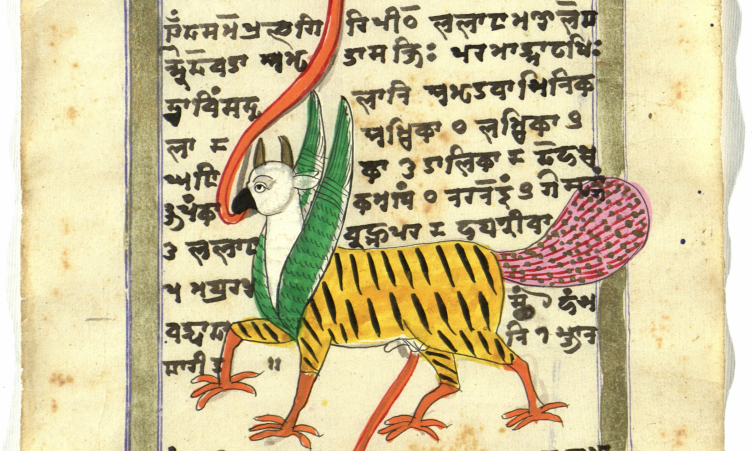
\includegraphics[width=1\textwidth]{pics/Wolpertinger.png}
\caption[The \textit{dehasvarūpa} of \textit{ajapāgāyatrī}]{The \textit{dehasvarūpa} of \textit{ajapāgāyatrī}. The image, reminiscent of a hippogriff, is part of an illustrated Sanskrit manuscript written in the Śāradā script. Preserved as a single large scroll under Acc. No. 1334 at the Oriental Institute in Srinagar (Kashmir), it is entitled \textit{Nāḍīcakra}. The manuscript contains a depiction of the yogic body’s \textit{cakra}s and \textit{nāḍī}s. The text surrounding the figure closely corresponds to the additional material found in manuscript \getsiglum{U2} of the \textit{Tattvayogabindu}. The manuscript reads (diplomatic transcription): \textit{oṃ daśame pūrṇagiripīṭhe lalāṭamaṇḍale candro devatā amṛtāśaktiḥ paramātmā ṛṣiḥ dvāviṃśaddalāni amṛtavāsinikalā 4: ambikā 1 lambikā 2 gha(ṃ)ṭkā 3 tālikā 4 dehasvarūpaṃ kākamukhaṃ 1 naranetraṃ 2 gośṛṅgaṃ 3 lalāṭabrahmapara 4 hayagrīvā 5 mayūramuśchaṃ 6 haṃsacārītani 7 sthāna.}}
	\phantomsection\label{fig_wolpertinger}
      \end{figure}

      \clearpage

  \begin{figure}[ht]
	\centering
  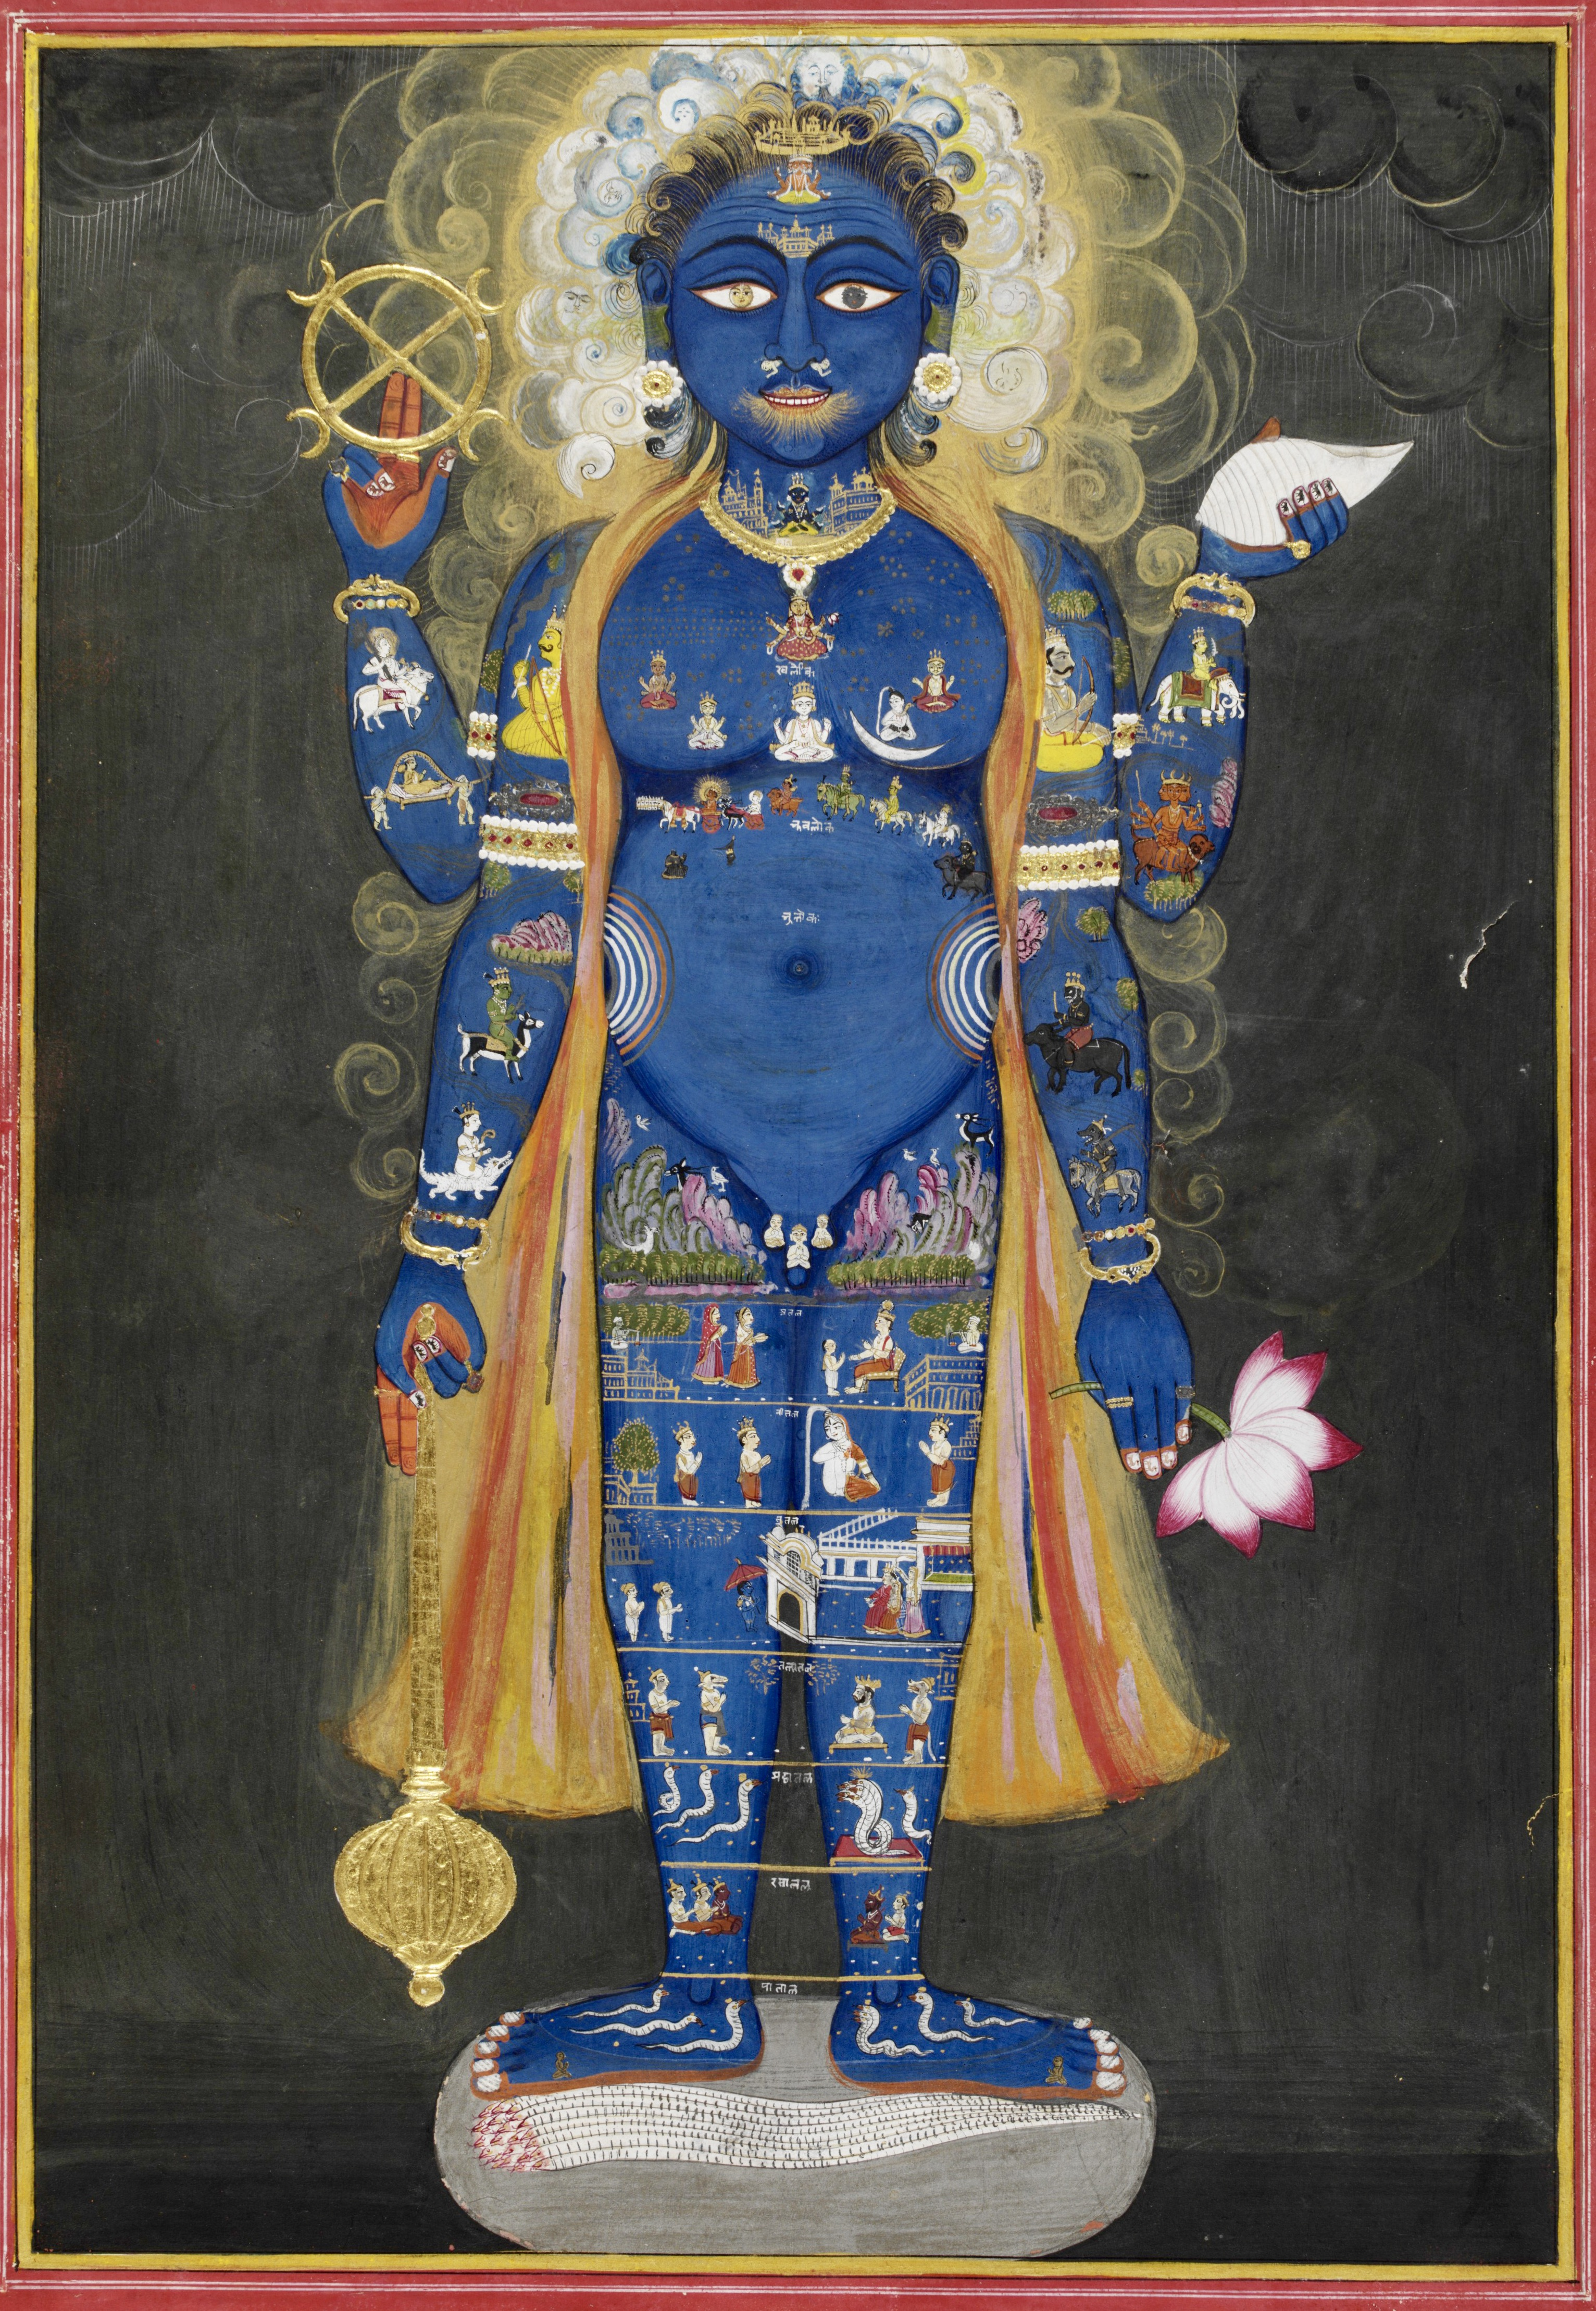
\includegraphics[width=1\textwidth]{pics/Vishnu_Vishvarupa_cropped.jpg}
	\caption{Viṣṇu Viśvarūpa, India, Rajasthan, Jaipur, ca. 1800–1820, Opaque watercolor and gold on paper, 38.5 × 28 cm, Victoria and Albert Museum, London, Given by Mrs. Gerald Clark.}
	\label{fig1}
      \end{figure}
\clearpage
  \begin{figure}[ht]
	\centering
  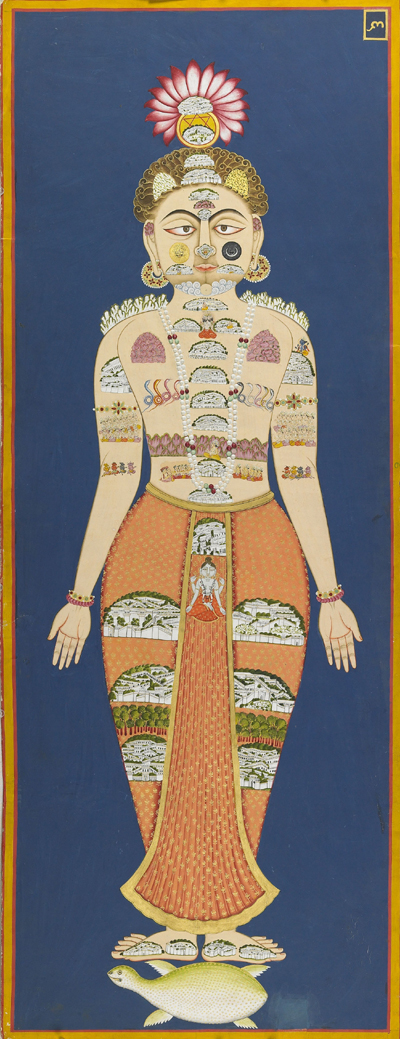
\includegraphics[width=0.5\textwidth]{pics/The_Equivalence_of_Self_and_Universe_(detail),_folio_6_from_the_Siddha_Siddhanta_Paddhati,_(Bulaki),_1824_(Samvat_1881);_122_x_46_cm._Mehrangarh_Museum_Trust..jpg}
	\caption{The Equivalence of Self and Universe (detail), folio 6 from the \textit{Siddhasiddhāntapaddhati} (Bulaki), India, Rajasthan, Jodhpur, 1824 (Samvat 1881), 122 x 46 cm, RJS 2378, Mehragarh Museum Trust.}
	\label{fig2}
      \end{figure}
      % \end{landscape}

      \newpage
      \cleardoublepage
\chapter{Bibliography}
 \label{sec:bibli}
\clearpage
\newpage 
\thispagestyle{empty}
\quad  \addtocounter{page}{-1}

\newrefcontext[sorting=tixel]
\printbibliography[heading=subbibintoc, title=Primary Sources, keyword=primary]

\newrefcontext[sorting=nyt]
\printbibliography[heading=subbibintoc, title=Secondary Literature, keyword=seclit]

\printbibliography[heading=subbibintoc, title=Catalogues, keyword=catalogues]

\printbibliography[heading=subbibintoc, title=Online Sources, keyword=onlinesource]

\end{document}


%%% Local Variables:
%%% mode: latex
%%% TeX-master: t
%%% End:
